% !TeX program = xelatex
\documentclass[10pt]{beamer}

\usetheme{metropolis}

\usepackage{pgfplots}
\usepgfplotslibrary{fillbetween}
\usepackage{pgfopts}
\usepackage{amsmath}
\usepackage{structuralanalysis}
\usepackage{tikz}
\usepackage{tikz-3dplot}
\usepackage{chngcntr}
\usepackage{wasysym}
\usepackage{mathtools}
\usepackage{alphalph}
\usepackage{xcolor}
\usepackage[showdow=false, en-US]{datetime2}

\newcommand{\highlight}[1]{%
	\colorbox{red!50}{$\displaystyle#1$}}

\setcounter{lecture}{11}
\counterwithin{equation}{lecture}
\makeatletter
\def\user@resume{resume}
\def\user@intermezzo{intermezzo}
%
\newcounter{previousequation}
\newcounter{lastsubequation}
\newcounter{savedparentequation}
\setcounter{savedparentequation}{1}
% 
\renewenvironment{subequations}[1][]{%
	\def\user@decides{#1}%
	\setcounter{previousequation}{\value{equation}}%
	\ifx\user@decides\user@resume 
	\setcounter{equation}{\value{savedparentequation}}%
	\else  
	\ifx\user@decides\user@intermezzo
	\refstepcounter{equation}%
	\else
	\setcounter{lastsubequation}{0}%
	\refstepcounter{equation}%
	\fi\fi
	\protected@edef\theHparentequation{%
		\@ifundefined {theHequation}\theequation \theHequation}%
	\protected@edef\theparentequation{\theequation}%
	\setcounter{parentequation}{\value{equation}}%
	\ifx\user@decides\user@resume 
	\setcounter{equation}{\value{lastsubequation}}%
	\else
	\setcounter{equation}{0}%
	\fi
	\def\theequation  {\theparentequation  \alph{equation}}%
	\def\theHequation {\theHparentequation \alph{equation}}%
	\ignorespaces
}{%
%  \arabic{equation};\arabic{savedparentequation};\arabic{lastsubequation}
\ifx\user@decides\user@resume
\setcounter{lastsubequation}{\value{equation}}%
\setcounter{equation}{\value{previousequation}}%
\else
\ifx\user@decides\user@intermezzo
\setcounter{equation}{\value{parentequation}}%
\else
\setcounter{lastsubequation}{\value{equation}}%
\setcounter{savedparentequation}{\value{parentequation}}%
\setcounter{equation}{\value{parentequation}}%
\fi\fi
%  \arabic{equation};\arabic{savedparentequation};\arabic{lastsubequation}
\ignorespacesafterend
}
\makeatother
\title{AE 737 - Mechanics of Damage Tolerance}
\subtitle{Lecture \arabic{lecture}}
\date{Last Updated: \today\ at \DTMcurrenttime}
\author{Dr. Nicholas Smith}
\institute{Wichita State University, Department of Aerospace Engineering}
% \titlegraphic{\hfill\includegraphics[height=1.5cm]{logo/logo}}

\begin{document}

\maketitle
\begin{frame}{schedule}
	\begin{itemize}
		\item 25 Feb - Multiple Site Damage, Mixed-mode Fracture, Homework 4 Due, Homework 5 Assigned
		\item 1 Mar - Section 1 Review, Homework 5 Due
		\item 3 Mar - Section 1 Review, Homework 5 return
		\item 8 Mar - Exam 1
		\item 10 Mar - Exam return, Final Project discussion
	\end{itemize}
\end{frame}

\begin{frame}{$a$ vs. $a_{eff}$}
	\begin{itemize}[<+->]
		\item When do we / don't we need to include effects of plastic zone size?
		\item Ductile/tough material vs. brittle/stiff material?
		\item Plane stress vs. plane strain?
		\item Charts/FE data
	\end{itemize}
\end{frame}

\begin{frame}
  \frametitle{outline}
  \setbeamertemplate{section in toc}[sections numbered]
  \tableofcontents[hideallsubsections]
\end{frame}

\section{stiffener review}

\begin{frame}{stiffeners}
	\begin{itemize}[<+->]
		\item Stiffener charts were made using physical crack length (not effective crack length)
		\item As cracks get long, the relative difference between $a$ and $a_{eff}$ is minor
		\item An active field of research is to integrate failsafes and crack stoppers in one part
		\item Manufacturing methods for composites are very different than for metals and damage tolerant designs need to adjust
	\end{itemize}
\end{frame}

\begin{frame}{stiffeners}
	\begin{itemize}
		\item Group 1 - Sketch and describe the effect of crack stoppers on panel residual strength
		\item Group 2 - Sketch a residual strength curve for a typical stiffened panel and describe how to find regions of stable and un-stable crack growth.
		\item Group 3 - Describe the effect of stiffener cross-sectional area using the figure on p. 186
		\item Group 4 - What does the text mean when it says unstable cracking will begin at shorter crack lengths?
	\end{itemize}
\end{frame}

\section{multiple site damage}

\begin{frame}{multiple site damage}
	\begin{itemize}[<+->]
		\item Often damage can accumulate among multiple sources
		\item This is very common when there are a series of holes, each can develop cracks with a potential to link up
		\item "link up" occurs when the plastic zones between two adjacent cracks touch
	\end{itemize}
\end{frame}

%TODO redo figure
\begin{frame}{linkup}
\begin{figure}
\centering
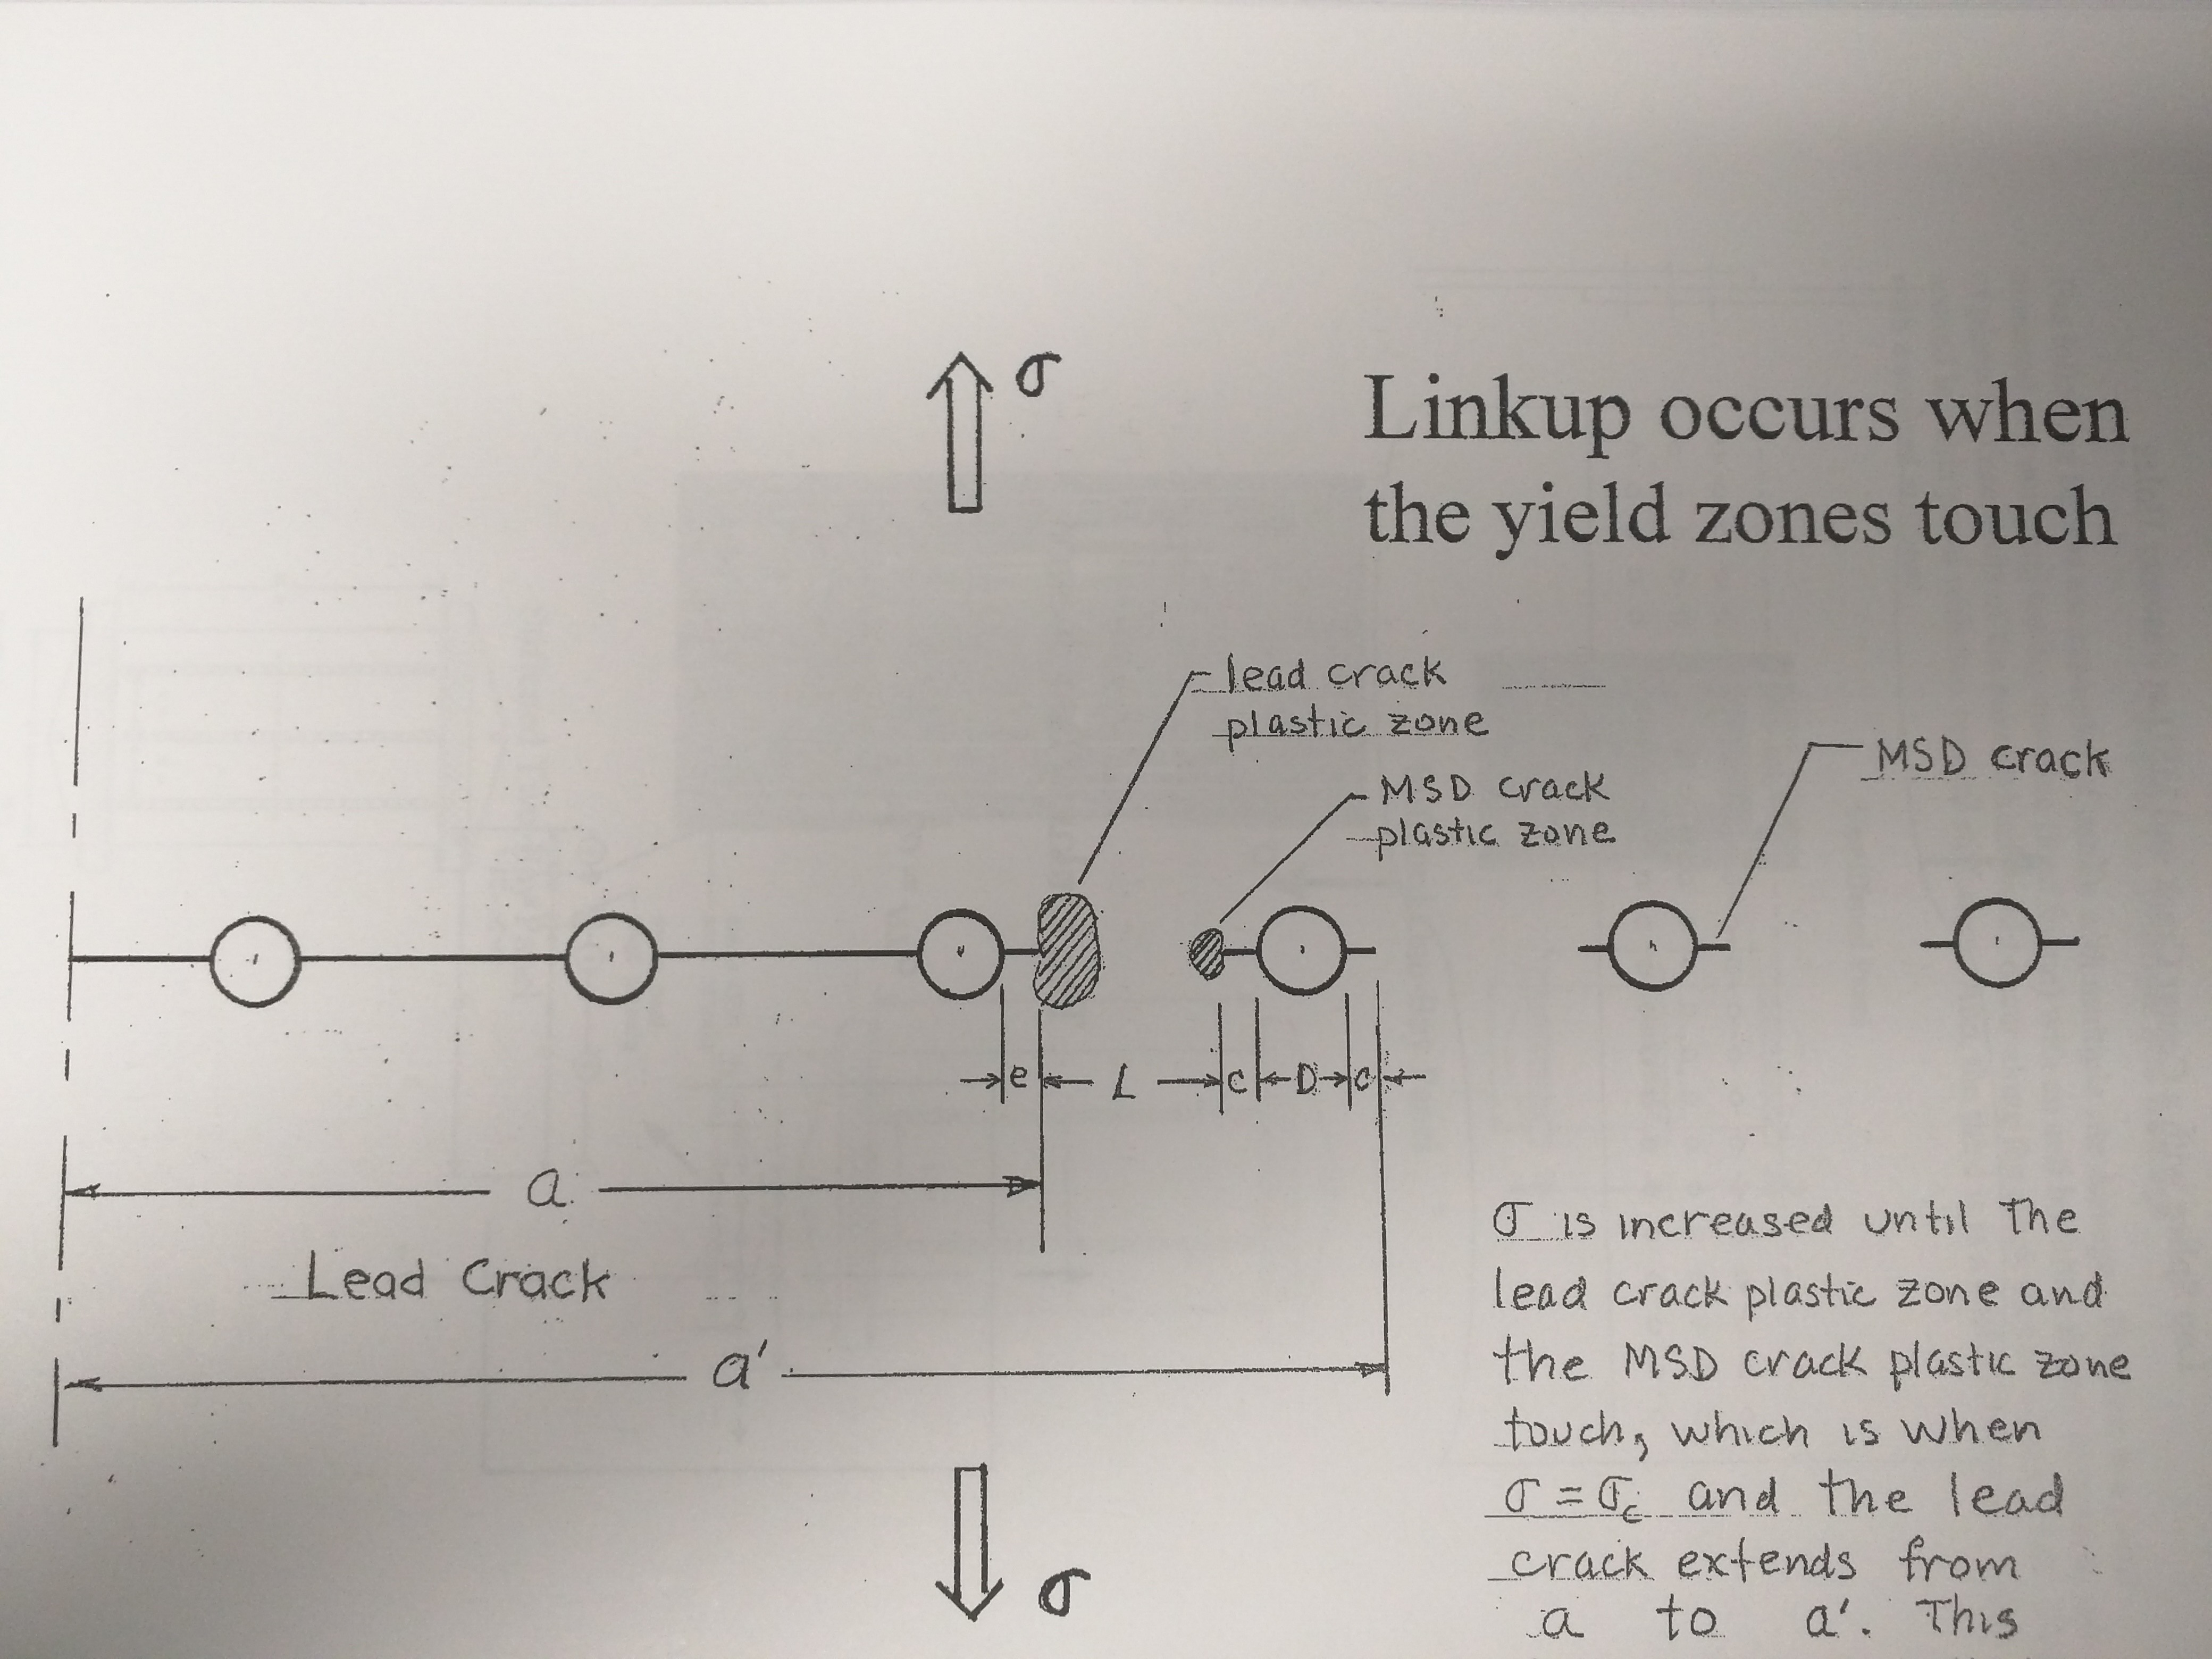
\includegraphics[width=0.7\linewidth]{msd}
\label{fig:msd}
\end{figure}
\end{frame}

%TODO redo figure
\begin{frame}{linkup}
\begin{figure}
\centering
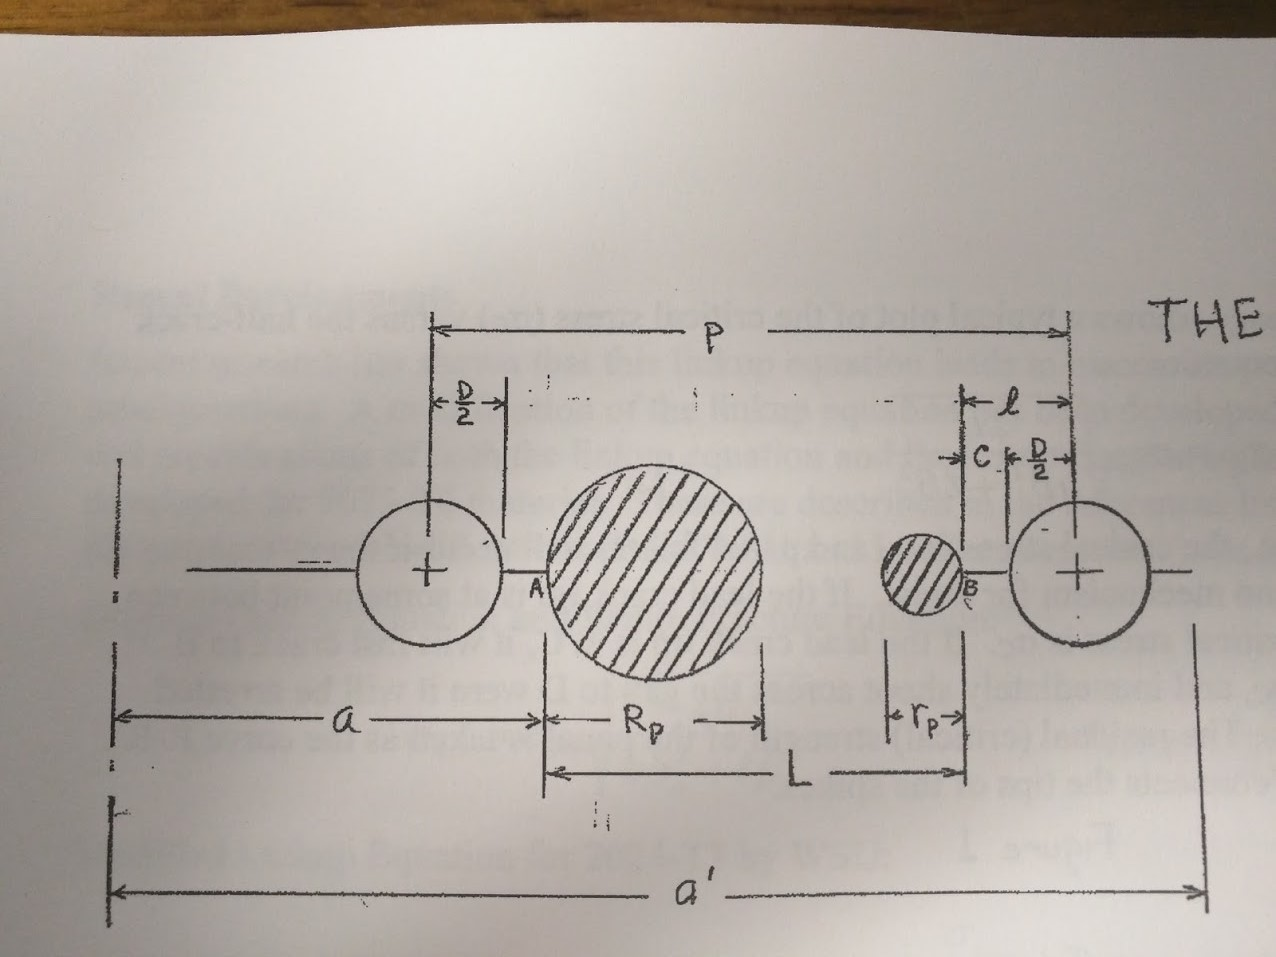
\includegraphics[width=0.7\linewidth]{linkup}
\label{fig:linkup}
\end{figure}
\end{frame}

\begin{frame}{linkup equation}
	\begin{itemize}[<+->]
		\item We know that
		\begin{equation}
		R_p = \frac{1}{2\pi}\left(\frac{K_{Ia}}{\sigma_{YS}}\right)^2
		\end{equation}
		\begin{equation}
		r_p = \frac{1}{2\pi}\left(\frac{K_{Il}}{\sigma_{YS}}\right)^2
		\end{equation}
		\item Where we define the stress intensity factors at a and L as
		\begin{equation}
		K_{Ia} = \sigma \sqrt{\pi a} \beta_a
		\end{equation}
		\begin{equation}
		K_{Il} = \sigma \sqrt{\pi l} \beta_l
		\end{equation}
	\end{itemize}
\end{frame}

\begin{frame}{linkup equation}
	\begin{itemize}[<+->]
		\item Since fast cracking occurs when $R_p + r_p = L$, we solve for the condition where $R_p + r_p < L$
		\begin{subequations}
		\begin{align}
		\frac{1}{2\pi}\left(\frac{K_{Ia}}{\sigma_{YS}}\right)^2 + \frac{1}{2\pi}\left(\frac{K_{Il}}{\sigma_{YS}}\right)^2 &< L\\
		\frac{1}{2\pi\sigma_{YS}^2} \left[K_{Ia}^2 + K_{Il}^2\right] &< L \\
		\frac{1}{2\pi\sigma_{YS}^2} \left[\sigma^2 \pi a \beta_a^2 + \sigma^2 \pi l \beta_l^2\right] &< L \\
		\frac{\sigma^2}{2\sigma_{YS}^2} \left[a \beta_a^2 + l \beta_l^2\right] &< L \\
		\frac{\sigma_c^2}{2\sigma_{YS}^2} \left[a \beta_a^2 + l \beta_l^2\right] &= L \\
		\label{eq:msd}
		\sigma_c &= \sigma_{YS}\sqrt{\frac{2L}{a \beta_a^2 + l \beta_l^2}}
		\end{align}
		\end{subequations}
	\end{itemize}
\end{frame}

\begin{frame}<handout:0>{example}
	
\end{frame}

\begin{frame}{modfied linkup equations}
	\begin{itemize}[<+->]
		\item We see that for a brittle material (with a small plastic zone) we predict no effect of "link-up"
		\item This does not agree with test data
		\item Even the 2024 predictions don't agree well with test data
		\item WSU used some empirical parameters to modify the linkup equations and better predict residual strength when multiple site damage is present
	\end{itemize}
\end{frame}

\begin{frame}{modified 2024 equation}
	\begin{itemize}[<+->]
		\item For 2024-T3 we use the following procedure
		\item First find $\sigma_c$ from (~\ref{eq:msd})
		\item[]
		\begin{equation}
		\sigma_{c,mod} = \frac{\sigma_c}{A_1 \ln (L) + A_2}
		\end{equation}
		\item Where $A_1 = 0.3065$ and $A_2 = 1.3123$ for A-basis yield strength and $A_1 = 0.3054$ and $A_2 = 1.3502$ for B-basis yield strength
		\item The same equation can also be used for 2524 with $A_1 = 0.1905$, $A_2 = 0.9683$ for A-basis yield and $A_1 = 0.2024$, $A_2 = 1.0719$ for B-basis yield
	\end{itemize}
\end{frame}

\begin{frame}{modified 7075 equations}
	\begin{itemize}[<+->]
		\item A similar modification was made for 7075
		\item[] \begin{equation}
		\sigma_{c,mod} = \frac{\sigma_c}{B_1 + B_2 L}
		\end{equation}
		\item Where $B_1 = 1.377$, $B_2 = 1.042$ for A-basis yield strength and $B_1 = 1.417$, $B_2 = 1.073$ for B-basis yield strength
		\item However, since general fracture had a closer prediction to real failure than the linkup equation, it may make more sense to modify the brittle fracture equation
		\item[]
		\begin{equation}
		\sigma_{c,mod} = \frac{K_c}{\sqrt{\pi a} (0.856 - 0.496 \ln(L))}
		\end{equation}
	\end{itemize}
\end{frame}

\begin{frame}<handout:0>{example}
\end{frame}

\section{mixed mode fracture}

\begin{frame}{mixed-mode fracture}
	\begin{itemize}[<+->]
		\item Most cracks are primarily Mode I, but sometimes Mode II can also have an effect
		\item We can look at the combined stress field for Mode I and Mode II
		\item Recall the stress field near the crack tip
		\begin{subequations}
		\begin{align}
		\sigma_x &= \frac{K_I}{\sqrt{2\pi r}} \cos \frac{\theta}{2} \left(1-\sin \frac{\theta}{2}\sin \frac{3\theta}{2}\right)\\
		\sigma_y &= \frac{K_I}{\sqrt{2\pi r}} \cos \frac{\theta}{2} \left(1+\sin \frac{\theta}{2}\sin \frac{3\theta}{2}\right)\\
		\tau_{xy} &= \frac{K_I}{\sqrt{2\pi r}} \sin \frac{\theta}{2} \cos \frac{\theta}{2}\cos \frac{3\theta}{2}
		\end{align}
		\end{subequations}
	\end{itemize}
\end{frame}

\begin{frame}{mixed-mode fracture}
	\begin{itemize}[<+->]
		\item For Mode II we have
		\item[]
		\begin{subequations}
			\begin{align}
			\sigma_x &= \frac{-K_{II}}{\sqrt{2\pi r}} \sin \frac{\theta}{2} \left(2+\cos \frac{\theta}{2}\cos \frac{3\theta}{2}\right)\\
			\sigma_y &= \frac{K_{II}}{\sqrt{2\pi r}} \sin \frac{\theta}{2} \cos \frac{\theta}{2}\cos \frac{3\theta}{2}\\
			\tau_{xy} &= \frac{K_{II}}{\sqrt{2\pi r}} \cos \frac{\theta}{2} \left(1-\sin \frac{\theta}{2}\sin \frac{3\theta}{2}\right)
			\end{align}
		\end{subequations}
	\end{itemize}
\end{frame}

\begin{frame}{polar coordinates}
	\begin{itemize}[<+->]
		\item In mixed-mode fracture problems, the crack will generally propagate in a different direction from the initial crack plane
		\item It is more convenient to handle this scenario in Polar Coordinates
		\item We can convert stress from Cartesian coordinates to Polar Coordinates using the stress transformation equations
		\item[]
		\begin{subequations}
			\begin{align}
		\sigma_r &= \sigma_x \cos^2 \theta + \sigma_y \sin^2 \theta + 2\tau_{xy} \sin \theta \cos \theta\\
		\sigma_\theta &= \sigma_x \sin^2 \theta + \sigma_y \cos^2 \theta - 2\tau_{xy} \sin \theta \cos \theta\\
		\tau_{r\theta} &= -\sigma_x \sin \theta \cos \theta + \sigma_y \sin \theta \cos \theta + \tau_{xy} (\cos^\theta - \sin^2 \theta)
		\end{align}
		\end{subequations}
	\end{itemize}
\end{frame}

\begin{frame}{combined stress field}
	\begin{itemize}[<+->]
		\item When we convert the stress fields from Mode I and Mode II into polar coordinates and combine them, we find
		\item[]
		\begin{subequations}
			\begin{align}
			\sigma_r &= \frac{K_I}{\sqrt{2\pi r}} \left(\frac{5}{4}\cos \frac{\theta}{2} - \frac{1}{4}\cos \frac{3\theta}{2}\right) + \frac{K_{II}}{\sqrt{2\pi r}}\left(-\frac{5}{4}\sin \frac{\theta}{2} + \frac{3}{4}\sin \frac{3\theta}{2}\right)\\
			\label{eq:mixed-theta}
			\sigma_\theta &= \frac{K_I}{\sqrt{2\pi r}} \left(\frac{3}{4}\cos \frac{\theta}{2} + \frac{1}{4}\cos \frac{3\theta}{2}\right) + \frac{K_{II}}{\sqrt{2\pi r}}\left(-\frac{3}{4}\sin \frac{\theta}{2} - \frac{3}{4}\sin \frac{3\theta}{2}\right)\\
			\label{eq:mixed-tau}
			\tau_{r\theta} &= \frac{K_I}{\sqrt{2\pi r}} \left(\frac{1}{4}\sin \frac{\theta}{2} + \frac{1}{4}\sin \frac{3\theta}{2}\right) + \frac{K_{II}}{\sqrt{2\pi r}}\left(\frac{1}{4}\cos \frac{\theta}{2} + \frac{3}{4}\cos \frac{3\theta}{2}\right)
			\end{align}
		\end{subequations}
	\end{itemize}
\end{frame}

\begin{frame}{maximum circumferential stress criterion}
	\begin{itemize}[<+->]
		\item The Maximum Circumferential Stress Criterion assumes that a crack will propagate in the principal direction
		\item In this direction, the shear stress is 0
		\item The fracture toughness is determined by the Mode I fracture toughness of the material
		\item \textbf{Note:} In this discussion, we will use $K_{IC}$ to differentiate Mode I fracture toughness from Mode II fracture toughness. This does NOT necessarily mean we are referring to plane strain fracture toughness
		\item Thus fracture begins when
		\begin{equation}
		\sigma_{\theta}(\theta_P) = \sigma_\theta(\theta=0, K_{II}=0, K_I = K_{Ic}) = \frac{K_{IC}}{\sqrt{2\pi r}}
		\end{equation}
	\end{itemize}
\end{frame}

\begin{frame}{maximum circumferential stress criterion}
	\begin{itemize}[<+->]
		\item Following the above assumptions, we can solve Equations~\ref{eq:mixed-tau} and~\ref{eq:mixed-theta} to find $\theta_P$
		\item Note: This assumes that we know both $K_I$ and $K_{II}$, in this class we have not discussed any Mode II stress intensity factors, so they will be given.
		\item Equation~\ref{eq:mixed-tau} in this case simplifies to
		\begin{equation}
		K_I \sin \theta_p + K_{II} (3\cos \theta_P -1) = 0
		\end{equation}
		\item and Equation~\ref{eq:mixed-theta} simplifies to
		\begin{equation}
		4K_{IC} = K_I\left(3\cos \frac{\theta}{2} + \cos \frac{3\theta}{2}\right) - 3K_{II}\left(\sin \frac{\theta}{2} + \sin \frac{3\theta}{2}\right)
		\end{equation}
		\item The general form for a Mode II stress intensity factor is
		\item[]
		\begin{equation}
		K_{II} = \tau \sqrt{\pi a} \beta^\prime
		\end{equation}
	\end{itemize}
\end{frame}

\begin{frame}{example}
	\begin{figure}[H]
		Assuming $|\sigma| = 4|\tau|$, $K_{IC} = 60 \text{ ksi} \sqrt{\text{in}}$, and $2a = 1.5 \text{ in}$.
		
		\textbf{Note:} Assume $\beta = \beta^\prime = 1$
		
		\centering
		\begin{tikzpicture}
		\draw (0,-2) -- (0,2) -- (4,2) -- (4,-2) -- (0,-2);
		\draw (1.5,0) -- (2.5,0);
		\draw[->] (2,2.5) -- (2,3) node[above] {$\sigma$};
		\draw[->] (2,-2.5) -- (2,-3) node[below] {$\sigma$};
		\draw[->] (1,2.2) -- (3,2.2);
		\draw[->] (3,-2.2) -- (1,-2.2);
		\draw[->] (4.2,-1) -- (4.2,1);
		\draw[->] (-0.2,1) -- (-0.2,-1);
		\draw node at (4.2,2.2) {$\tau$};
		\draw node at (-0.2,-2.2) {$\tau$};
		\draw node at (2,0.2) {$2a$};
		\end{tikzpicture}
	\end{figure}
\end{frame}

\begin{frame}{principal stress criterion}
	\begin{itemize}[<+->]
		\item In the maximum circumferential stress criterion, we found the principal direction in polar coordinates
		\item We can also find the principal direction in Cartesian coordinates
		\item If we make a free body cut along some angle $\theta$ we find, from equilibrium
		\item[]
		\begin{subequations}
			\begin{align}
			0 &= \sigma_\theta dA - \sigma_x dA \sin^2 \theta - \sigma_y dA \cos^2 \theta + 2\tau_{xy} dA \cos \theta \sin \theta\\
			\sigma_\theta &= \sigma_x \sin^2 \theta + \sigma_y \cos^2 \theta - 2 \tau_{xy} \sin \theta \cos \theta\\
			\frac{\partial \sigma_\theta}{\partial \theta} &= (\sigma_x - \sigma_y) \sin 2\theta_p - 2\tau_{xy} \cos 2\theta_P\\
			\tan 2\theta_P &= \frac{2 \tau_{xy}}{\sigma_x - \sigma_y}
			\end{align}
		\end{subequations}
	\end{itemize}
\end{frame}

\begin{frame}{principal stress criterion}
	\begin{itemize}[<+->]
		\item As before, we consider crack propagation purely due to Mode I
		\item In the principal stress criterion, we find the maximum Mode I stress as a function of the remote applied stress
		\begin{equation}
		\sigma_{P1} = C \sigma
		\end{equation}
		\item We then find the remote failure stress by
		\begin{equation}
		\sigma_c = \frac{K_{IC}}{C\sqrt{\pi a}\beta}
		\end{equation}
	\end{itemize}
\end{frame}

\begin{frame}{example}
	\begin{figure}[H]
		Assuming $|\sigma| = 4|\tau|$, $K_{IC} = 60 \text{ ksi} \sqrt{\text{in}}$, and $2a = 1.5 \text{ in}$.
		
		\textbf{Note:} Assume $\beta = \beta^\prime = 1$
		
		\centering
		\begin{tikzpicture}
		\draw (0,-2) -- (0,2) -- (4,2) -- (4,-2) -- (0,-2);
		\draw (1.5,0) -- (2.5,0);
		\draw[->] (2,2.5) -- (2,3) node[above] {$\sigma$};
		\draw[->] (2,-2.5) -- (2,-3) node[below] {$\sigma$};
		\draw[->] (1,2.2) -- (3,2.2);
		\draw[->] (3,-2.2) -- (1,-2.2);
		\draw[->] (4.2,-1) -- (4.2,1);
		\draw[->] (-0.2,1) -- (-0.2,-1);
		\draw node at (4.2,2.2) {$\tau$};
		\draw node at (-0.2,-2.2) {$\tau$};
		\draw node at (2,0.2) {$2a$};
		\end{tikzpicture}
	\end{figure}
\end{frame}
\end{document}
